\begin{frame}
    \begin{centering}
        \vskip5ex plus 1filll
        {\usebeamerfont{title page title}\usebeamercolor[fg]{title page} Building Blocks\\[1.5ex]}
        \vskip0pt plus 1filll
    \end{centering}
\end{frame}

\begin{frame}{What is a nonlinear system?}
    Frequency domain: you get out more than what you put in
    \begin{figure}
        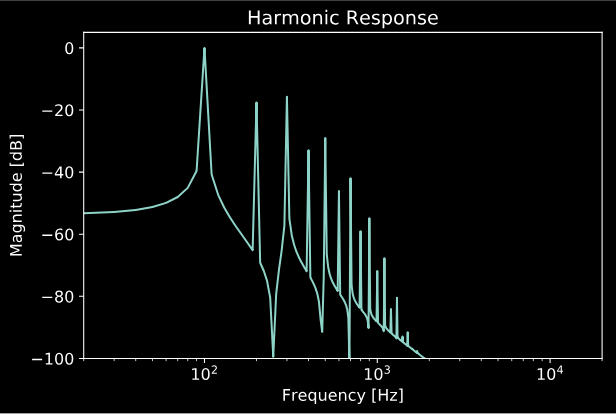
\includegraphics[width=3.75in]{../Exciter/Pics/exciter_harm.png}
    \end{figure}
\end{frame}

\begin{frame}{What is a nonlinear system?}
    Time domain: static response
    \begin{figure}
        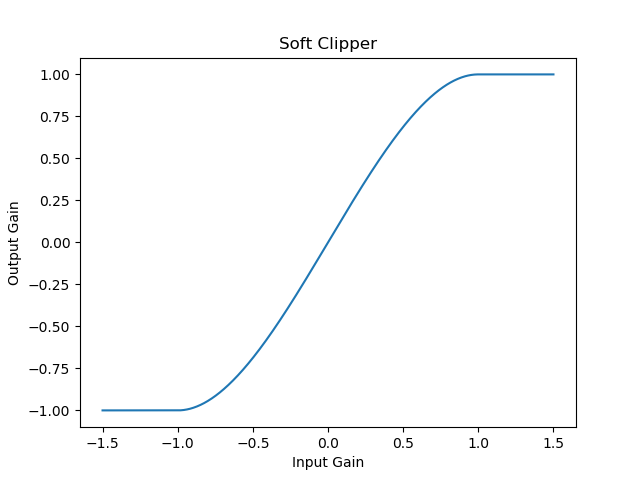
\includegraphics[height=2.5in]{../DoubleSoftClipper/Pics/SC.png}
    \end{figure}
\end{frame}

\begin{frame}{What is a nonlinear system?}
    Time domain: dynamic response
    \begin{figure}
        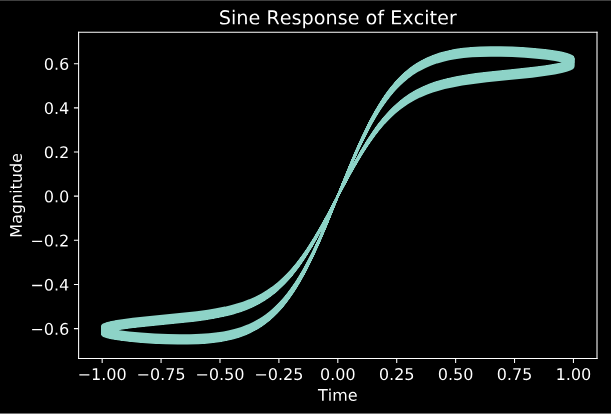
\includegraphics[width=3.75in]{../Exciter/Pics/exciter_static.png}
    \end{figure}
\end{frame}

\begin{frame}{Saturating Nonlinearities}
    \begin{figure}
        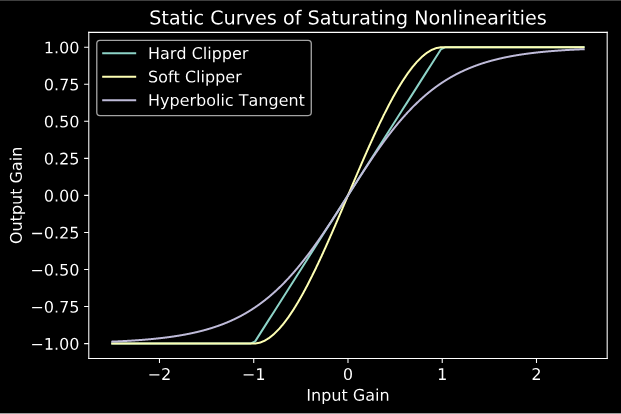
\includegraphics[width=3.75in]{../Exciter/Pics/saturating_static.png}
    \end{figure}
\end{frame}

\begin{frame}{Rectifying Nonlinearities}
    \begin{figure}
        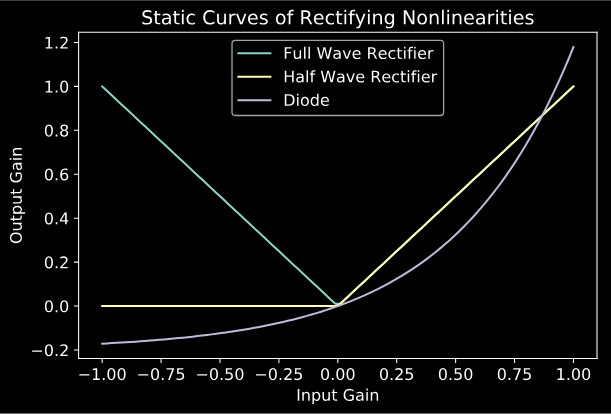
\includegraphics[width=3.75in]{../Exciter/Pics/rect_static.png}
    \end{figure}
\end{frame}

\begin{frame}{Dropout Nonlinearities}
    \begin{figure}
        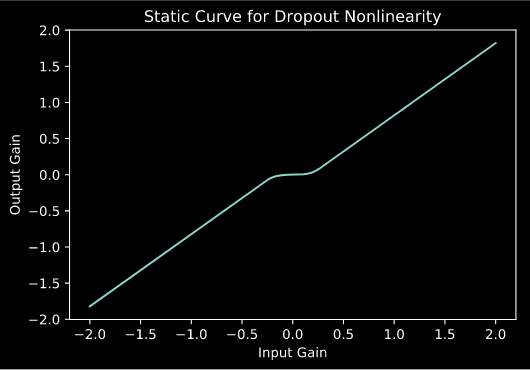
\includegraphics[width=3.5in]{../Paper/Pics/dropout.png}
    \end{figure}

    \begin{center}
        \scriptsize (also called ``dead-zone'')
    \end{center}
\end{frame}

\begin{frame}{What is a ``Complex Nonlinearity''}
    Has one of the following properties:\newline
    \begin{itemize}
        \item Is not memoryless (has some memory of past states)
        \item Has an interesting harmonic response
        \item Has interesting parameters
    \end{itemize}
\end{frame}
